% This LaTeX was auto-generated from MATLAB code.
% To make changes, update the MATLAB code and export to LaTeX again.

\documentclass{article}

\usepackage[utf8]{inputenc}
\usepackage[T1]{fontenc}
\usepackage{lmodern}
\usepackage{graphicx}
\usepackage{color}
\usepackage{hyperref}
\usepackage{amsmath}
\usepackage{amsfonts}
\usepackage{epstopdf}
\usepackage[table]{xcolor}
\usepackage{matlab}

\sloppy
\epstopdfsetup{outdir=./}
\graphicspath{ {./README_RST_images/} }

\matlabhastoc

\begin{document}

\label{T_0B344E76}
\matlabtitle{Color Performance Review Tool for Endoscopy Devices - User's Manual}

\matlabtableofcontents{Table of Contents}
\label{H_0BBD90AF}
\matlabheading{1. Introduction}

\begin{par}
\begin{flushleft}
The Color Performance Review (CPR) Tool for Endoscopy Devices is a software program written in Matlab for analyzing color performance testing data in endoscopy device. The tool accepts the testing data and then generates quantitative analyses for the user to compare color performance between devices. The input testing data include the measurement data of a standard test target from the device output as well as the ground truth of the test target. 
\end{flushleft}
\end{par}

\begin{par}
\begin{flushleft}
The tool provides the following analyses: 
\end{flushleft}
\end{par}

\begin{itemize}
\setlength{\itemsep}{-1ex}
   \item{\begin{flushleft} Visual simulation of the test target and sample scenes \end{flushleft}}
   \item{\begin{flushleft} Absolute color errors in comparison with the ground truth \end{flushleft}}
   \item{\begin{flushleft} Preservation of the patch order in lightness, hue, and chroma \end{flushleft}}
   \item{\begin{flushleft} Preservation of color contrast between patches \end{flushleft}}
\end{itemize}

\label{H_58570BBF}
\matlabheadingtwo{1.1 Software Requirements}

\begin{itemize}
\setlength{\itemsep}{-1ex}
   \item{\begin{flushleft} Matlab Runtime 9.12 (Version 9.12 tested) \end{flushleft}}
   \item{\begin{flushleft} Matlab (Version 9.12 tested) \end{flushleft}}
   \item{\begin{flushleft} Image Processing Toolbox (Version 11.5 tested) \end{flushleft}}
   \item{\begin{flushleft} Computer Vision Toolbox (Version 9.12 tested) \end{flushleft}}
   \item{\begin{flushleft} Statistics and Machine Learning Toolbox (Version 12.3 tested) \end{flushleft}}
\end{itemize}

\label{H_9F32CBC1}
\matlabheading{2. Data Processing}

\label{H_2D2A9D19}
\matlabheadingtwo{2.0 Data Preparation}

\begin{par}
\begin{flushleft}
The input data should include the measured CIEXYZ values of the 24-patch \href{https://www.xrite.com/categories/calibration-profiling/colorchecker-classic-family/colorchecker-classic-nano}{ColorChecker} for the test target and the endoscopy device. The input files are text files in the comma-separated value (CSV) format. Each input file contains 25 rows of the CIE X, Y, and Z values separated by commas. Lines \#1\textasciitilde{}\#24 describe the 24 color patches, and Line \#25 describes the reference white. Follow the patch order defined by the ColorChecker.
\end{flushleft}
\end{par}

\begin{par}
\begin{flushleft}
The following is a sample input file:
\end{flushleft}
\end{par}

\begin{matlabcode}
type('XYZ_Subject.csv')
\end{matlabcode}
\begin{matlaboutput}
19.1,16.2,8.9
76.6,72.2,58.4
40.6,41.7,80.7
20.1,26.4,9.8
61.3,58.6,99.5
80.7,95,106.7
66.8,58.4,12.1
24.5,20.3,77.6
47.3,29.1,24.3
5.5,3.3,12.1
66.5,85.1,19.3
74.1,74.9,11.2
10.8,6.8,46
29.3,46.6,15.1
29.2,16.4,5.3
95,107.4,14.7
56.4,38,69.2
44.2,51.1,100.4
167.3,174.2,193.4
124.8,130.3,145.4
88.1,92.2,103.4
45.2,47.3,52.6
13.6,14.2,17.4
0.6,0.6,0.8
167.3,174.2,193.4
\end{matlaboutput}

\begin{par}
\begin{flushleft}
\textit{Figure 2.0: CIEXYZ input file. A sample input file of the CIEXYZ data measured from the device.}
\end{flushleft}
\end{par}

\label{H_A03EC777}
\matlabheadingtwo{2.1 Import Data}

\begin{par}
\begin{flushleft}
Provide filenames for loading data files that contain the measured CIEXYZ values of the 24-patch ColorChecker for the test target (e.g., 'XYZ\_Reference.csv') and the subject device (e.g., 'XYZ\_Subject.csv'): 
\end{flushleft}
\end{par}

\begin{matlabcode}
XYZ_Reference_filename = "XYZ_Reference.csv";
XYZ_Reference = csvread(XYZ_Reference_filename);

XYZ_Subject_filename = "XYZ_Subject.csv";
XYZ_Subject = csvread(XYZ_Subject_filename);
\end{matlabcode}

\label{H_3F7B7B2D}
\matlabheadingtwo{2.2 CIEXYZ Data}

\begin{par}
\begin{flushleft}
The input data for the ground truth (\texttt{Ref\_X}, \texttt{Ref\_Y}, and \texttt{Ref\_Z}) and endoscopy device (\texttt{Sub\_X}, \texttt{Sub\_Y}, and \texttt{Sub\_Z}) are combined into \texttt{CIEXYZ\_Data} as a 25x6 table for inspection:
\end{flushleft}
\end{par}

\begin{matlabcode}
% create a table to show the data

Ref_X = XYZ_Reference(:,1);
Ref_Y = XYZ_Reference(:,2);
Ref_Z = XYZ_Reference(:,3);

Sub_X = XYZ_Subject(:,1);
Sub_Y = XYZ_Subject(:,2);
Sub_Z = XYZ_Subject(:,3);

CIEXYZ_Data = table(Ref_X,Ref_Y,Ref_Z,Sub_X,Sub_Y,Sub_Z)
\end{matlabcode}
\begin{matlabtableoutput}
{
\begin{tabular} {|c|c|c|c|c|c|c|}\hline
\mlcell{ } & \mlcell{Ref\_X} & \mlcell{Ref\_Y} & \mlcell{Ref\_Z} & \mlcell{Sub\_X} & \mlcell{Sub\_Y} & \mlcell{Sub\_Z} \\ \hline
\mlcell{1} & \mlcell{51.1000} & \mlcell{46.2000} & \mlcell{32.2000} & \mlcell{19.1000} & \mlcell{16.2000} & \mlcell{8.9000} \\ \hline
\mlcell{2} & \mlcell{149.7000} & \mlcell{139.3000} & \mlcell{108.5000} & \mlcell{76.6000} & \mlcell{72.2000} & \mlcell{58.4000} \\ \hline
\mlcell{3} & \mlcell{69.4000} & \mlcell{73.2000} & \mlcell{144.7000} & \mlcell{40.6000} & \mlcell{41.7000} & \mlcell{80.7000} \\ \hline
\mlcell{4} & \mlcell{47} & \mlcell{59.4000} & \mlcell{31} & \mlcell{20.1000} & \mlcell{26.4000} & \mlcell{9.8000} \\ \hline
\mlcell{5} & \mlcell{103.7000} & \mlcell{97.5000} & \mlcell{190} & \mlcell{61.3000} & \mlcell{58.6000} & \mlcell{99.5000} \\ \hline
\mlcell{6} & \mlcell{125.6000} & \mlcell{171} & \mlcell{189.6000} & \mlcell{80.7000} & \mlcell{95} & \mlcell{106.7000} \\ \hline
\mlcell{7} & \mlcell{160.1000} & \mlcell{131.2000} & \mlcell{31.4000} & \mlcell{66.8000} & \mlcell{58.4000} & \mlcell{12.1000} \\ \hline
\mlcell{8} & \mlcell{52.6000} & \mlcell{43.9000} & \mlcell{164.4000} & \mlcell{24.5000} & \mlcell{20.3000} & \mlcell{77.6000} \\ \hline
\mlcell{9} & \mlcell{110.9000} & \mlcell{72.8000} & \mlcell{58} & \mlcell{47.3000} & \mlcell{29.1000} & \mlcell{24.3000} \\ \hline
\mlcell{10} & \mlcell{25.5000} & \mlcell{17.4000} & \mlcell{44.5000} & \mlcell{5.5000} & \mlcell{3.3000} & \mlcell{12.1000} \\ \hline
\mlcell{11} & \mlcell{129.1000} & \mlcell{171.9000} & \mlcell{41.2000} & \mlcell{66.5000} & \mlcell{85.1000} & \mlcell{19.3000} \\ \hline
\mlcell{12} & \mlcell{169.1000} & \mlcell{159} & \mlcell{24.7000} & \mlcell{74.1000} & \mlcell{74.9000} & \mlcell{11.2000} \\ \hline
\mlcell{13} & \mlcell{29.1000} & \mlcell{21.7000} & \mlcell{105.1000} & \mlcell{10.8000} & \mlcell{6.8000} & \mlcell{46} \\ \hline
\mlcell{14} & \mlcell{56.8000} & \mlcell{94.1000} & \mlcell{39.6000} & \mlcell{29.3000} & \mlcell{46.6000} & \mlcell{15.1000} \\ 
\hline
\end{tabular}
}
\end{matlabtableoutput}

\begin{par}
\begin{flushleft}
\textit{Figure 2.2: Verification of the input data. The CIEXYZ data of the ground truth (first three columns) and the device output (last three columns).}
\end{flushleft}
\end{par}

\label{H_3BA7C911}
\matlabheadingtwo{2.3 CIELAB Data}

\begin{par}
\begin{flushleft}
The CIEXYZ data are converted into CIELAB data:
\end{flushleft}
\end{par}

\begin{matlabcode}
% create the DeviceData objects
LAB_Reference = CPR.DeviceData;
LAB_Reference.setXYZ(XYZ_Reference);

LAB_Subject = CPR.DeviceData;
LAB_Subject.setXYZ(XYZ_Subject);

% create an object of the ColorPerformaneReview class
cpr = CPR.ColorPerformanceReview(LAB_Reference,LAB_Subject);
\end{matlabcode}

\begin{par}
\begin{flushleft}
Show the CIELAB data for the user to examine:
\end{flushleft}
\end{par}

\begin{matlabcode}
% create a table to show the data
Ref_L_star = LAB_Reference.Lab(:,1);
Ref_a_star = LAB_Reference.Lab(:,2);
Ref_b_star = LAB_Reference.Lab(:,3);

Sub_L_star = LAB_Subject.Lab(:,1);
Sub_a_star = LAB_Subject.Lab(:,2);
Sub_b_star = LAB_Subject.Lab(:,3);

CIELAB_Data = table(Ref_L_star,Ref_a_star,Ref_b_star,Sub_L_star,Sub_a_star,Sub_b_star)
\end{matlabcode}
\begin{matlabtableoutput}
{
\begin{tabular} {|c|c|c|c|c|c|c|}\hline
\mlcell{ } & \mlcell{Ref\_L\_star} & \mlcell{Ref\_a\_star} & \mlcell{Ref\_b\_star} & \mlcell{Sub\_L\_star} & \mlcell{Sub\_a\_star} & \mlcell{Sub\_b\_star} \\ \hline
\mlcell{1} & \mlcell{43.0069} & \mlcell{13.4819} & \mlcell{13.7046} & \mlcell{36.5549} & \mlcell{16.0282} & \mlcell{18.9414} \\ \hline
\mlcell{2} & \mlcell{69.2457} & \mlcell{15.7802} & \mlcell{14.9991} & \mlcell{70.4877} & \mlcell{12.5809} & \mlcell{14.9385} \\ \hline
\mlcell{3} & \mlcell{52.7901} & \mlcell{0.0828} & \mlcell{-26.6662} & \mlcell{56.0257} & \mlcell{1.4192} & \mlcell{-25.2700} \\ \hline
\mlcell{4} & \mlcell{48.1630} & \mlcell{-16.1059} & \mlcell{23.7018} & \mlcell{45.8458} & \mlcell{-19.8571} & \mlcell{32.6213} \\ \hline
\mlcell{5} & \mlcell{59.6874} & \mlcell{12.8386} & \mlcell{-28.5801} & \mlcell{64.6754} & \mlcell{10.0484} & \mlcell{-21.1622} \\ \hline
\mlcell{6} & \mlcell{75.2755} & \mlcell{-31.9891} & \mlcell{-1.5924} & \mlcell{78.7727} & \mlcell{-16.3737} & \mlcell{-0.6324} \\ \hline
\mlcell{7} & \mlcell{67.5603} & \mlcell{31.7213} & \mlcell{56.7733} & \mlcell{64.5835} & \mlcell{20.8401} & \mlcell{59.5397} \\ \hline
\mlcell{8} & \mlcell{42.0110} & \mlcell{20.3700} & \mlcell{-51.5650} & \mlcell{40.6597} & \mlcell{19.3255} & \mlcell{-49.8244} \\ \hline
\mlcell{9} & \mlcell{52.6646} & \mlcell{50.7821} & \mlcell{11.2775} & \mlcell{47.8861} & \mlcell{52.7936} & \mlcell{9.9764} \\ \hline
\mlcell{10} & \mlcell{26.6127} & \mlcell{28.7565} & \mlcell{-24.5855} & \mlcell{14.9229} & \mlcell{26.8858} & \mlcell{-26.0821} \\ \hline
\mlcell{11} & \mlcell{75.4354} & \mlcell{-29.3516} & \mlcell{62.0779} & \mlcell{75.3591} & \mlcell{-26.1584} & \mlcell{64.7479} \\ \hline
\mlcell{12} & \mlcell{73.0884} & \mlcell{15.1033} & \mlcell{73.0162} & \mlcell{71.5526} & \mlcell{3.7517} & \mlcell{73.5749} \\ \hline
\mlcell{13} & \mlcell{29.8679} & \mlcell{24.2854} & \mlcell{-51.5005} & \mlcell{23.3500} & \mlcell{30.9640} & \mlcell{-56.0720} \\ \hline
\mlcell{14} & \mlcell{58.7972} & \mlcell{-44.9705} & \mlcell{34.6449} & \mlcell{58.7430} & \mlcell{-42.4243} & \mlcell{43.3861} \\ 
\hline
\end{tabular}
}
\end{matlabtableoutput}

\begin{par}
\begin{flushleft}
\textit{Figure 2.3: Verification of the color conversion. The converted CIELAB data of the ground truth (first three columns) and the device output (last three columns).}
\end{flushleft}
\end{par}

\label{H_604B1AFA}
\matlabheading{3. Data Analysis}

\label{H_8917CFBE}
\matlabheadingtwo{3.1 Visual simulation of the test target and sample scenes}

\label{H_EE44CB82}
\matlabheadingthree{3.1.1 Visualize CIEXYZ data}

\begin{par}
\begin{flushleft}
The following charts show the simulated visual results when using D65 as the reference white. Use these charts to check excessive color shift caused by the light source and/or the device.
\end{flushleft}
\end{par}

\begin{matlabcode}
if strcmp(cpr.devDataOriginal.source,'XYZ')
    cpr.evaluate_visual_XYZ;
end
\end{matlabcode}
\begin{center}
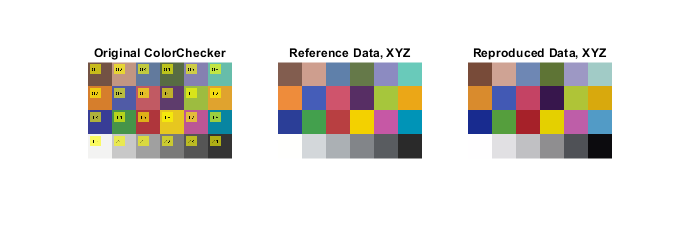
\includegraphics[width=\maxwidth{67.83743100852986em}]{figure_0.png}
\end{center}

\begin{par}
\begin{flushleft}
\textit{Figure 3.1.1: Visual verification of the CIEXYZ data. The charts show the simulated visual results when using D65 as the reference white. Use these charts to check excessive color shift caused by the light source and/or the device. }
\end{flushleft}
\end{par}


\label{H_9C6F9CA6}
\matlabheadingthree{3.1.2 Visualize CIELAB data}

\begin{par}
\begin{flushleft}
The following charts show the simulated visual results when using the provided reference white. Use these charts to assess how the device would reproduce the ColorChecker.
\end{flushleft}
\end{par}

\begin{matlabcode}
cpr.check_Lab_visual
\end{matlabcode}
\begin{center}
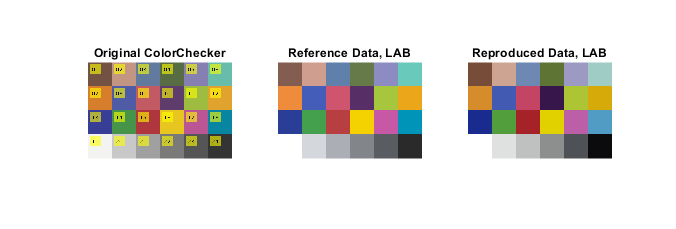
\includegraphics[width=\maxwidth{67.83743100852986em}]{figure_1.png}
\end{center}

\begin{par}
\begin{flushleft}
\textit{Figure 3.1.2: Visual verification of the CIELAB data. The charts show the simulated visual results when using the provided reference white. Use these charts to assess how the device would reproduce the test target.}
\end{flushleft}
\end{par}

\label{H_5E791428}
\matlabheadingthree{3.1.3 Visualize endoscopic scene}

\begin{par}
\begin{flushleft}
The following charts show the simulated visual results of an endoscopic scence. Use the default polyp sample or provide a different image according to the intended use.
\end{flushleft}
\end{par}

\begin{par}
\begin{flushleft}
Superficial esophageal cancer (type 0–IIa) is identified as slight reddish lesion
\end{flushleft}
\end{par}

\begin{matlabcode}
simulate_filename = "sample_polyp.png";
cpr.check_endoscopic_scene(simulate_filename);
\end{matlabcode}
\begin{center}
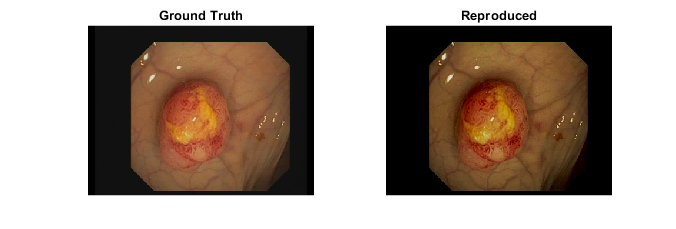
\includegraphics[width=\maxwidth{67.83743100852986em}]{figure_2.png}
\end{center}

\begin{par}
\begin{flushleft}
\textit{Figure 3.1.3: Visualize endoscopic scenes. The charts show the simulated visual results of an endoscopic scene. Use the default polyp sample or provide a different image according to the intended use.}
\end{flushleft}
\end{par}

\label{H_847C4C77}
\vspace{1em}


\label{H_91B3F5C5}
\matlabheadingtwo{3.2 Absolute color errors in comparison with the ground truth}

\begin{par}
\begin{flushleft}
The left chart shows the per-patch color difference between the endoscopy device and the ground truth. The right chart shows the boxplot. Statistics (mean, std, min, median, and max) are provided in the titles.
\end{flushleft}
\end{par}

\begin{matlabcode}
cpr.check_dE_from_truth
\end{matlabcode}
\begin{center}
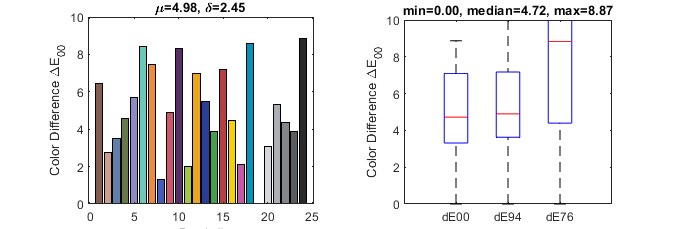
\includegraphics[width=\maxwidth{67.83743100852986em}]{figure_3.png}
\end{center}

\begin{par}
\begin{flushleft}
\textit{Figure 3.2: Absolute color errors in comparison with the ground truth. The left chart shows the per-patch color difference between the subject device and the ground truth. The right chart shows the box plot. The statistics (mean, standard deviation, minimum, median, and maximum) are provided in the titles.}
\end{flushleft}
\end{par}


\label{H_4AAE1EA7}
\matlabheadingtwo{3.3 Preservation of the patch order in lightness, hue, and chroma}

\label{H_20490D74}
\matlabheadingthree{3.3.1 Order in lightness, chroma, and hue - 1D view}

\begin{par}
\begin{flushleft}
The following charts show the patch order in lightness, chroma, and hue (1D view). The top row is the reference, the bottom row is the device output, and each line connects the same patch. Use these charts to identify any out-of-order patches and assess concordance and monotonicity.
\end{flushleft}
\end{par}

\begin{matlabcode}
cpr.check_order
\end{matlabcode}
\begin{center}
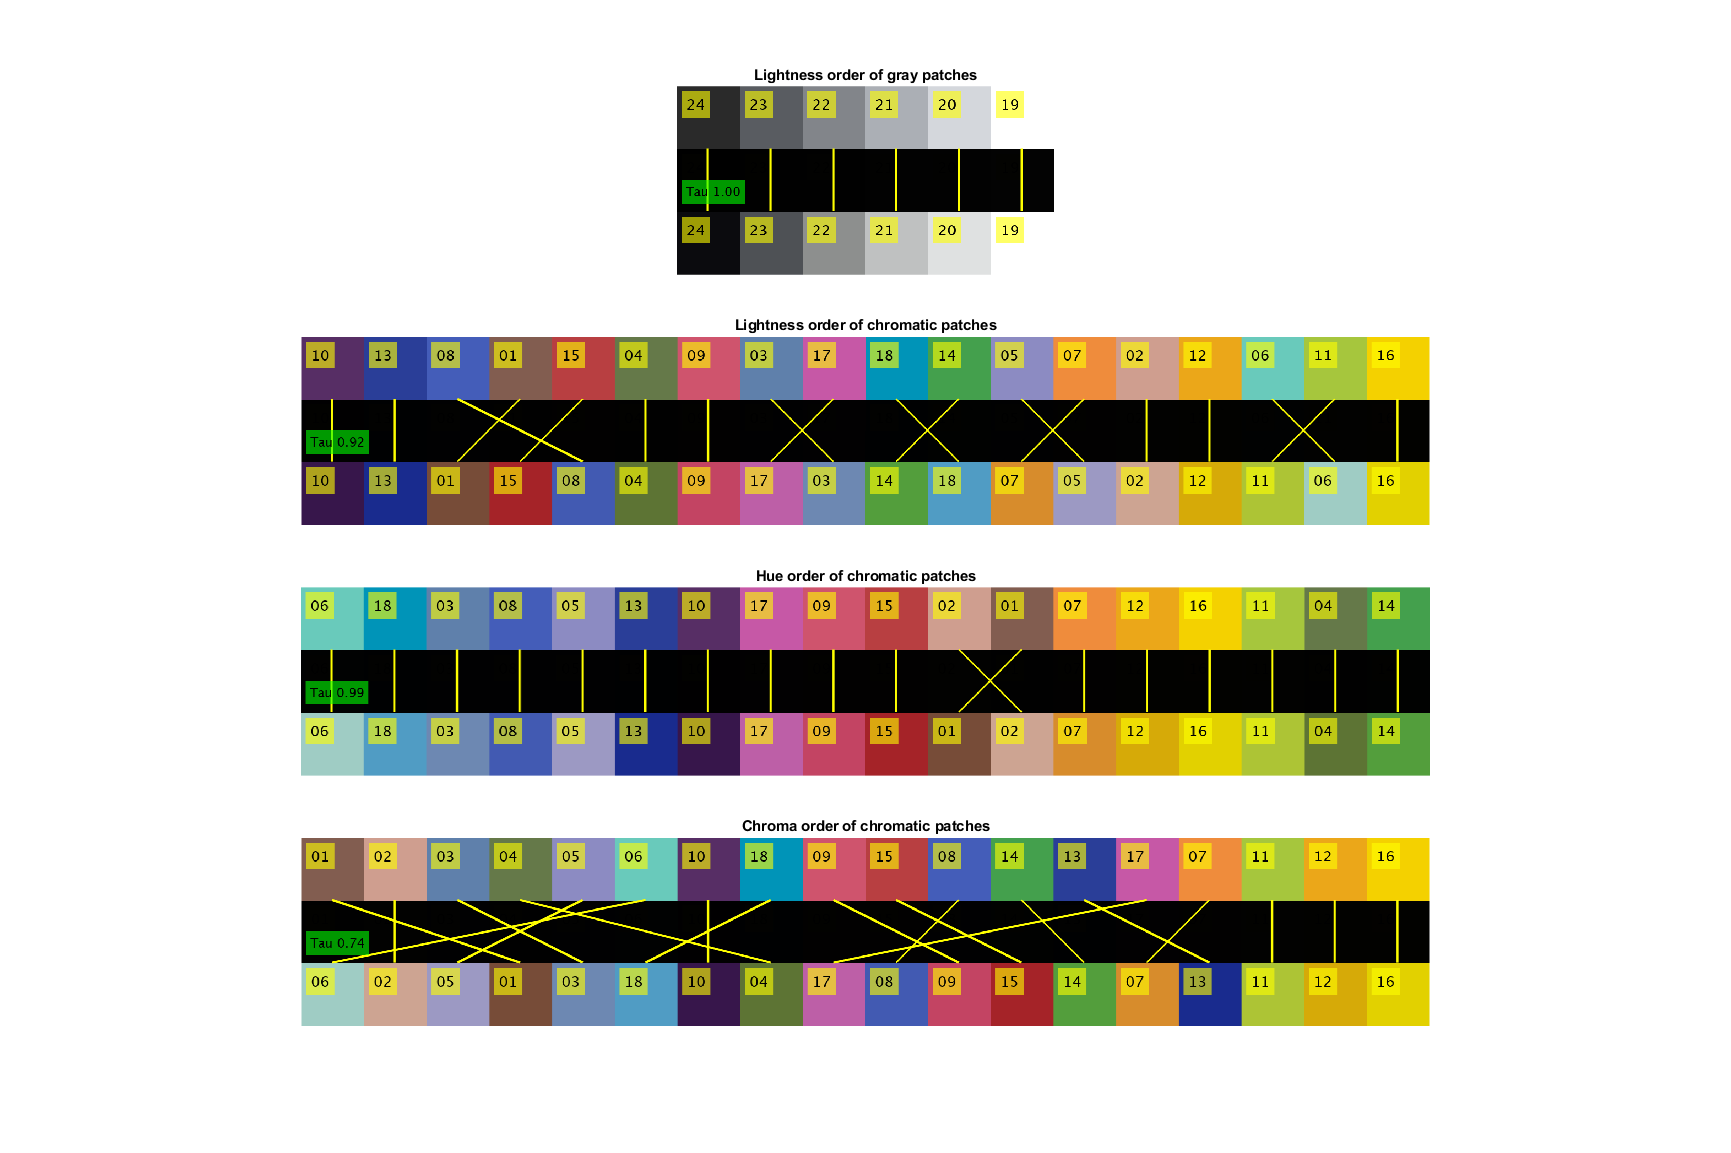
\includegraphics[width=\maxwidth{67.53637732062218em}]{figure_4.png}
\end{center}

\begin{par}
\begin{flushleft}
\textit{Figure 3.3.1: Preservation of the patch order in lightness/hue/chroma -- monotonicity. The charts show the patch order in lightness, chroma, and hue. In each chart, the top row is the reference, the bottom row is the device output, and each line connects the same patch. The top chart shows the patch order in lightness for gray patches (\#19-\#24). The remaining three charts show the chromatic patches in the lightness, hue, and chroma order. Use these charts to identify any out-of-order patches. The Kendall Tau-a rank correlation coefficients are included in each plot.}
\end{flushleft}
\end{par}


\label{H_D2C0E14C}
\matlabheadingthree{3.3.2 Order in lightness, chroma, and hue - 2D view}

\begin{par}
\begin{flushleft}
The following charts show the patch order in lightness, chroma, and hue (2D view). Use these charts to identify any out-of-order patches and assess linearity, concordance, and monotonicity.
\end{flushleft}
\end{par}

\begin{matlabcode}
cpr.check_linearity
\end{matlabcode}
\begin{matlaboutput}
Warning: Exported image displays axes toolbar. To remove axes toolbar from image, export again.
\end{matlaboutput}
\begin{center}
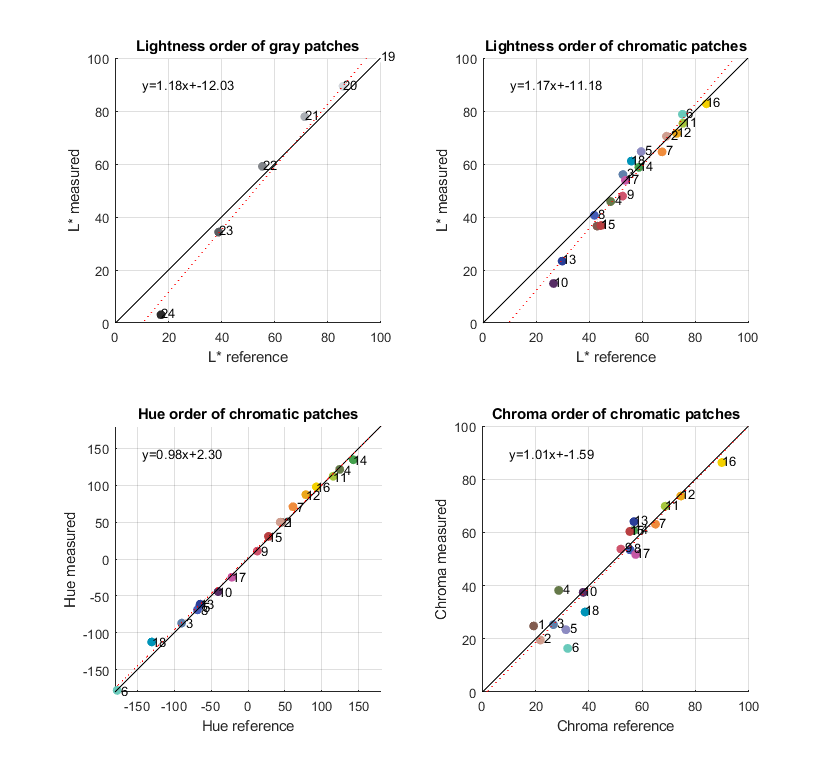
\includegraphics[width=\maxwidth{83.69292523833417em}]{figure_5.png}
\end{center}

\begin{par}
\begin{flushleft}
\textit{Figure 3.3.2: Preservation of the patch order in lightness/hue/chroma -- linearity. The top two charts show the patch order in lightness for gray patches (\#19-\#24) and chromatic patches (\#1-\#18). The lower left chart shows the chromatic patches in the hue order, and the lower right in the chroma order. Linear regression coefficients are included in each plot.}
\end{flushleft}
\end{par}


\label{H_804BFDA7}
\matlabheadingthree{3.3.3 Three-dimensional color transfer}

\begin{par}
\begin{flushleft}
The following charts show the color transfer from the ground truth (spheres) to the device output (crosses) of all patches in the CIELAB color space. Rotate the 3D plots in Matlab to observe the spatial relationship. 
\end{flushleft}
\end{par}

\begin{matlabcode}
cpr.check_color_transfer
\end{matlabcode}
\begin{center}
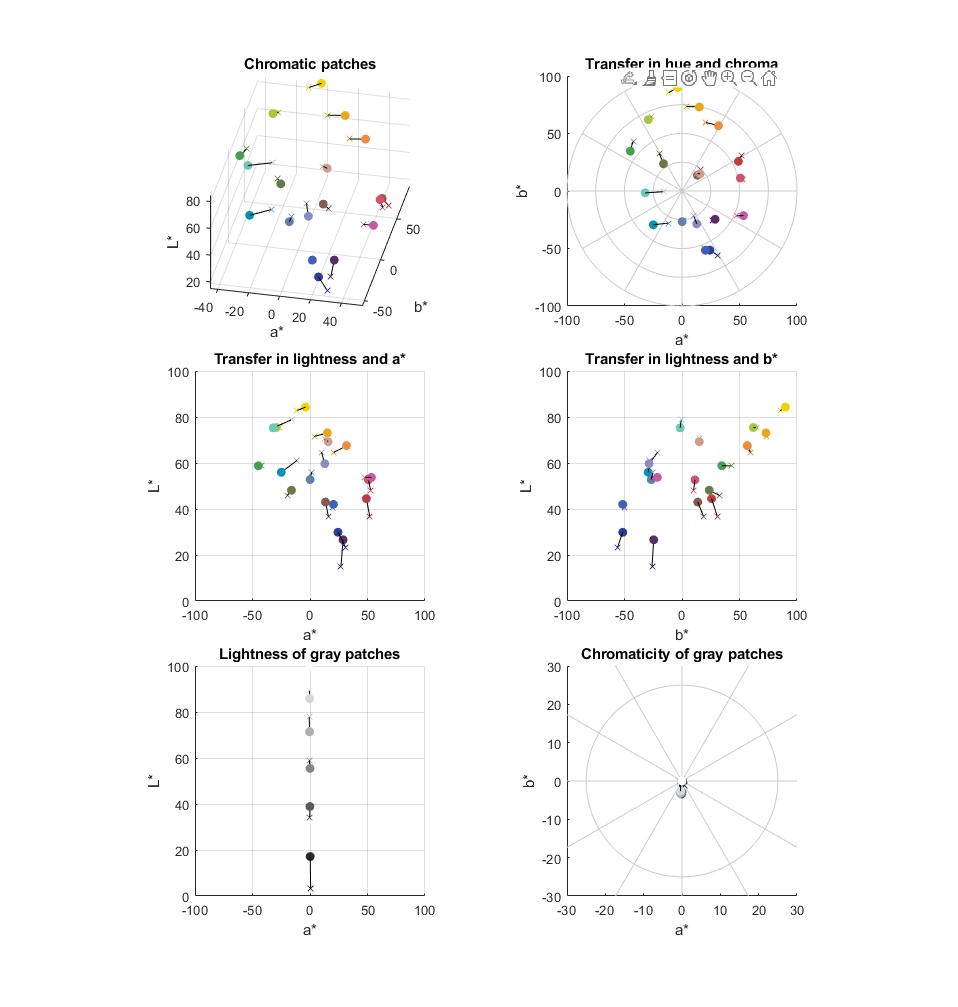
\includegraphics[width=\maxwidth{76.36728549924737em}]{figure_6.png}
\end{center}

\begin{par}
\begin{flushleft}
\textit{Figure 3.3.3: Visualization of color transfer. The top four charts show the color transfer of the chromatic patches observed from different angles. The bottom two charts show the color transfer of the gray patches to observe their lightness and chromaticity.}
\end{flushleft}
\end{par}


\label{H_E64AD261}
\matlabheadingtwo{3.4 Preservation of Color Contrast between Patches}

\begin{par}
\begin{flushleft}
The following charts show all datapoints plotted according to their ground truth and device output. The color contrast enhancement (CCE) is defined as follows:
\end{flushleft}
\end{par}

\begin{par}
\begin{flushleft}
$CCE=\frac{\Delta E(sub(i),sub(j))}{\Delta E(ref(i),ref(j))}$,
\end{flushleft}
\end{par}

\begin{par}
\begin{flushleft}
where $i$ and $j$ are patch numbers $1\le i\le 24,1\le j\le 24,i\not= j$. $ref(i)$ and $sub(i)$ are reference and subject device output for patch \#$i$, respectively. $\Delta E$ is a function calculating the CIE color difference between two colors based on either the $\Delta E_{00}$, $\Delta E_{94}$, or $\Delta E_{76}$ formulas.
\end{flushleft}
\end{par}

\begin{par}
\begin{flushleft}
$CCE=1$ (represented by the dotted red line) means that the device reproduces the color contrast perfectly. $CCE>1$ means that the device enhances the color contrast, while $CCE<1$ means otherwise.
\end{flushleft}
\end{par}

\begin{matlabcode}
cpr.check_cce
\end{matlabcode}

\begin{par}
\begin{flushleft}
\textit{Figure 3.4: Preservation of color contrast between patches. The CCE values calculated based on the }$\Delta E_{00}$\textit{, }$\Delta E_{94}$\textit{, or }$\Delta E_{76}$\textit{ formulas. Each colored cross represents a patch-pair where the horizontal and vertical bars are colored separately according to the patch-pair. The percentage indicates patch-pairs that have }$CCE\ge 1$\textit{.}
\end{flushleft}
\end{par}

\begin{matlabcode}
% close all figures
close all
\end{matlabcode}

\end{document}
